\chapter[Role of sills in the development of volcanic fields: Insights from lidar mapping surveys of the San Rafael Swell, Utah]{Role of sills in the development of volcanic fields: Insights from lidar mapping surveys of the San Rafael Swell, Utah \footnote{This chapter has been reprinted from Geology with permission from the Geological Society of America as: Richardson, J. A., Connor, C. B., Wetmore, P. E., Connor, L. C., and Gallant, E. A. (2015), Role of sills in the development of volcanic fields: Insights from lidar mapping surveys of the San Rafael Swell, Utah, Geology, 43(11), 1023-1026.}}\label{ch_sills}

%compile with pdflatex:
%:! bibtex %:r
%:! pdflatex -synctex=1 -interaction=nonstopmode --shell-escape %

\renewcommand*{\FigPath}{figures/chapter-sills}

\section{Abstract}

Analysis of airborne and terrestrial lidar data demonstrates that $>$0.4~km$^3$ of magma cooled in sills at shallow ($<$1~km) depth in the now eroded Pliocene San Rafael Swell distributed volcanic field, Utah (USA). The volumes of each of seven sills are estimated from 3D models of the lidar data and range from 10$^{-4}$-10$^{-1}$ km$^3$. Directions of magma flow during emplacement are interpreted from precise sill thickness measurements and measurements of linear vertical offsets within the sills, helping to identify feeder conduits and dikes; 3D map relationships derived from lidar data demonstrate that magma flowed into and out of sills from these active dikes and eruptive conduits. Mapped sill volumes account for $>$92\% of intrusive material within the 50~km$^2$ study area. We conclude that sills played a significant role in modifying eruption dynamics during activity in San Rafael, and suggest that monitoring of sill inflation and deflation in active distributed volcanic fields may provide key information about unrest and potential eruption dynamics.


\section{Introduction}

Intermediate to shallow crustal storage of pre- and syn-eruption magma modulates magma supply rate in many volcanic systems. At Mount St. Helens (A.D. 1980 eruption; USA) and Parícutin (A.D. 1943 eruption; Mexico), magma supply rate is thought to have been influenced by the presence of shallow ($<$10~km), temporary magma storage \citep{cashman2005multiple} and by the length of storage time \citep{scandone2007magma}. \citet{erlund2010compositional} identified increasing amounts of shallow crust ($\le$4 km depth) assimilated at Parícutin over the 9-year eruption, and concluded that a shallow intrusion network formed early and caused later eruptive products to be more effusive. On shorter timescales, gas may segregate preferentially into conduits above shallow sills, increasing volumetric flow in the conduit and intensifying the eruption \citep{conte2000experimental,pioli2009controls}. Sill-like intrusions into shallow magma chambers have recently been geodetically linked with interferometric synthetic aperture radar (InSAR) and seismic monitoring to eruptions at Tungurahua, Ecuador \citep{biggs2010stratovolcano} and Eyjafjallaj\"{o}kull, Iceland \citep{tarasewicz2012magma}. These models and observations suggest that it is critical to understand the volume, depth and distribution of sills in volcanic fields in order to forecast eruption dynamics and the evolution of volcanic systems. In young volcanic fields, such as the one around Parícutin \citep{connor1990cinder}, it is not possible to directly observe the shallow plumbing system. Here, we use lidar technology to map part of the eroded San Rafael Swell (UT) volcanic field. These data demonstrate that sills are prevalent at shallow depths ($<$1~km), modulated magma flow in eruptive conduits, and likely influenced eruption dynamics within this volcanic field.

\begin{figure}
\centering
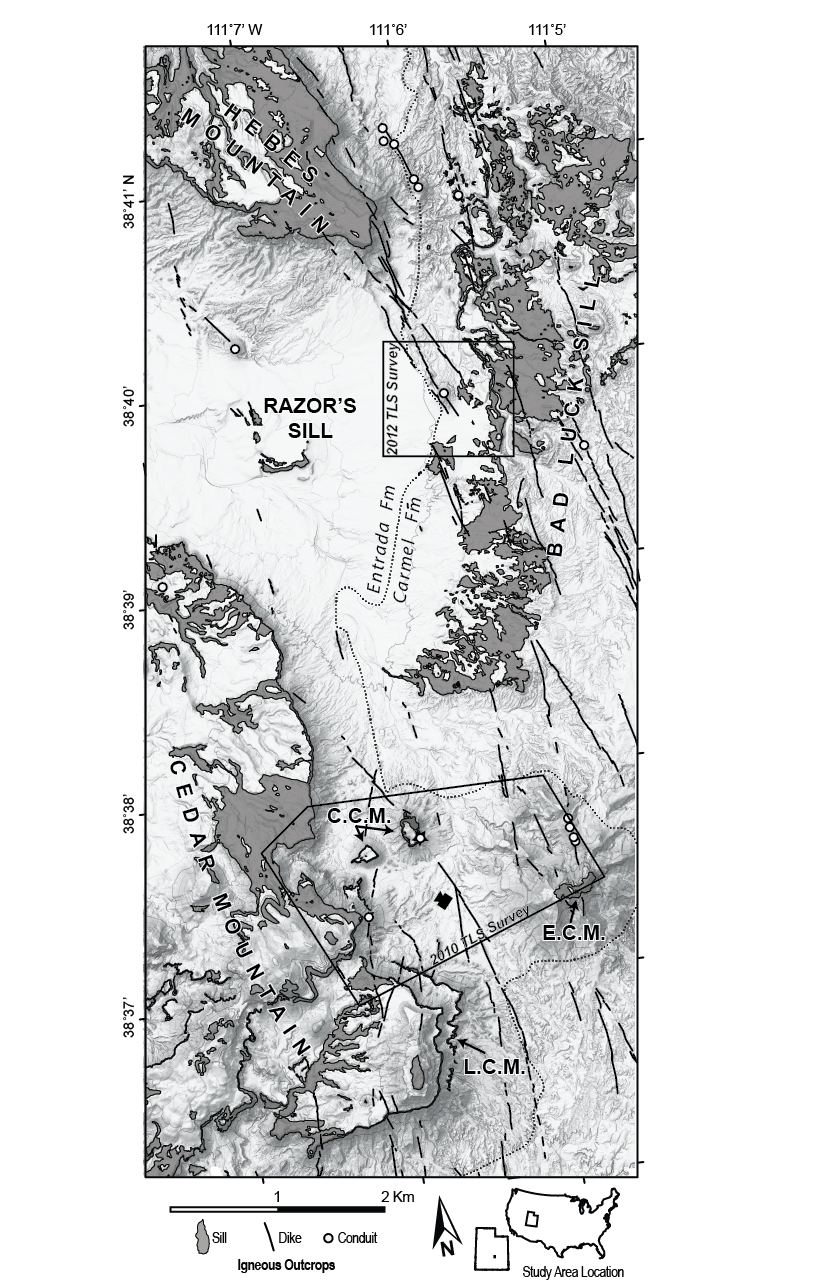
\includegraphics[width=0.4\linewidth]{\FigPath/Fig1-map}
\caption[Shaded relief map of airborne laser scanning data, San Rafael Swell, Utah (USA).]{Shaded relief map of airborne laser scanning data, San Rafael Swell, Utah (USA) with formation contact and terrestrial laser scanning (TLS) areas labeled. Sills mapped are Hebes, Bad Luck, Razor’s, Cedar Mountain, Lower Cedar Mountain (LCM), Central Cedar Mountain (CCM), and East Cedar Mountain (ECM). Starred conduit symbol near CCM denotes conduit that was formed concurrently with CCM sill. Camera symbol near CCM is view location of Figure \ref{fig_panorama}.}
\label{fig_map}
\end{figure}

\section{Geologic Description}

The San Rafael volcanic field was active between 4.6 and 3.8~Ma \citep{delaney1997physical}. This volcanic field is part of a larger occurrence of Cenozoic basaltic volcanism in the Colorado Plateau and Basin and Range provinces but is distinct from many other fields as it has been eroded to a depth of $\sim$800~m, based on its age and late Cenozoic erosion rates \citep[e.g.]{pederson2002colorado}. The sill-and-dike swarm, or volcanic plumbing system, cut a Jurassic sedimentary section from the Carmel Formation through the Cutler Formation. Diabasic dikes in this area trend 335$^{\circ}$ to 0$^{\circ}$ (relative to north) along regional joint sets, indicating low horizontal deviatoric stress during emplacement \citep{delaney1997physical}. Sills in the San Rafael Swell range from $<$5~m to $>$40~m thick and are exposed in cliff sides and canyons in outcrops that extend for 100s-1000s~m. This shallow magma plumbing system has been mapped \citep{delaney1997physical}, and used to improve our understanding of (i) dike emplacement \citep{delaney1986field}, (ii) magma diapirism in the shallow crust \citep{diez2009evidence}, and (iii) the spatial relationships between dikes and conduits \citep{kiyosugi2012relationship}, the latter of which are commonly surrounded by brecciated country rock, indicating conduit erosion during rapid magma ascent. Although \citet{gartner1986geometry} described physical characteristics of exposed sills in the area, the complex emplacement processes of sills in this volcanic field have remained enigmatic. With the aid of lidar, we are able to document the complex map relationships between intrusions in the area.

\section{Lidar Reconnaissance and Analysis}

Terrestrial laser scanning (TLS), performed in 2010 and 2012, collected a 7.3 GB point cloud over an area of 5 km$^2$. Both TLS surveys used Riegl terrestrial scanners. An airborne laser scanning (ALS) survey, in 2013, provided data for a 54 km$^2$ airborne laser swath map (ALSM) \citep{richardson2013alsm}, connecting the 2 TLS surveys into a single study area (Figure \ref{fig_map}). Instrument specifications and data formats from these surveys are outlined in Table \ref{tab_specifications}. Co-registering the coordinate systems of the three surveys creates a coverage area of $\sim$50~km$^2$, within which relief varies by up to 500~m. Thus, we are able to characterize the magma plumbing system in a tabular block approaching 25 km$^3$ in volume, which bounds the study area extent. This reconstruction of a magmatic plumbing system attempts to model the amount of magma emplaced into the crust due to Pliocene volcanism for the 25~km$^3$ space.

The three point clouds (two TLS and one ALSM) were consolidated and analyzed using LiDAR Viewer software \citep{kreylos2008immersive}. Because the three-dimensional point cloud is so precise, lidar data help identify subtle changes in sill thickness over large areas, vertical offsets in sills, and disrupted stratigraphy in overlying sedimentary units, which allow magma movements to be deduced. Contacts between igneous and sedimentary rocks are identified by shade contrast (igneous rocks are generally darker than sedimentary rocks in the near-infrared point cloud) and weathering patterns easily observable in the point cloud (Figure \ref{fig_photo-pcloud}). Thickness measurements are made in LiDAR Viewer where sill upper and lower contacts are seen in close proximity. The exact locations of sill contacts are manually picked between points in the point cloud, where one point is interpreted as sill and the other as sedimentary rock (Table 4). Uncertainty at each measurement is determined as the average of point-to-point distances on top and bottom of the sill and is drastically reduced in areas where both TLS and ALSM data are available. Other measurements made in LiDAR Viewer include sill base elevations and strikes and dips of continuous sill segments and of sedimentary host rock below sills. Locations where sills abruptly change stratigraphic level are also mapped in the field. These abrupt changes can be traced between outcrops with point cloud measurements.

Sill exposures are mapped using 1~m National Agriculture Imagery Program (NAIP) images and the ALSM digital elevation model (DEM). These are combined with thickness measurements to estimate terminal boundaries of sills. The lateral edges of sills are not commonly preserved in outcrop, so we have estimated the terminal boundary of each sill to extend no more than 0.5~km from current exposures. Sills commonly crop out at cliffs with little horizontal exposure area (Figure \ref{fig_panorama}), and by assuming that the mapped sills are contiguous between these outcrops, mapped sill areas are relatively small in comparison to interpreted sill areas (Table \ref{tab_mappedmodeled}). Sill volume and average thickness are modeled by constraining the thicknesses of sills at their respective modeled boundaries to be 0~m and interpolating a Laplacian-spline surface within sill boundaries, calibrated to the measured thicknesses (Figures \ref{fig_twomodels} and \ref{fig_fivemodels}). Results from mapped and modeled areas, and maximum measured thicknesses, are detailed in Table \ref{tab_mappedmodeled}.

Using aerial images and field mapping, \citet{kiyosugi2012relationship} mapped 16 conduits and ~180 vertical, en echelon dike segments, with a cumulative length of ~53 km, that crop out in the study area (Figure \ref{fig_map}). The cumulative volume of igneous material stored in dikes is estimated to be the product of dike length, the modeled block height, and 85 cm, the modal dike thickness \citep{delaney1997physical}. This might be a slight overestimate as some dikes might not have cut through the entire block height. The volume stored in conduits is the product of the surface area, mapped with the ALSM DEM and NAIP images, of each conduit and the modeled block height. This assumes conduit thickness does not change within the vertical limits of this reconstruction and might underestimate volume if conduits widen toward the surface or formed above the present-day surface.

\section{Igneous System Reconstruction}

\begin{figure}
\centering
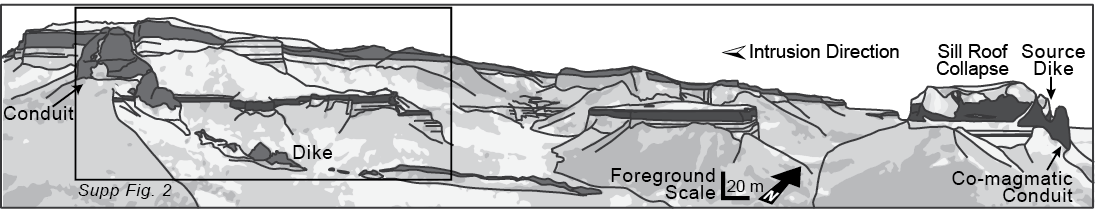
\includegraphics[width=\linewidth]{\FigPath/Fig2-panorama}
\caption[Northwest-facing panoramic diagram of Central Cedar sill]{Northwest-facing panoramic diagram of Central Cedar sill, shaded dark gray (see Figure \ref{fig_map} for location). Other igneous intrusions are lighter gray, including sill capping Cedar Mountain (background), a conduit, and a dike.}
\label{fig_panorama}
\end{figure}

\begin{table}
\centering
\caption{Areas, Thickness, and Volumes for 7 Sills in the Eroded San Rafael Swell Volcanic Field}
\begin{tabular}{p{3cm} c c | c c c}
\toprule
 & \multicolumn{2}{c}{Observations} & \multicolumn{3}{c}{Modeled values} \\ 
\midrule
 Sills & Mapped area$^*$ & Max  & Modeled area & Volume & Mean\\ 
 & (10$^3$ m$^2$) & thickness$^*$ & (10$^3$ m$^2$) & (km$^3$) & thickness\\
\midrule
Bad Luck & 2901$\pm$141 & 19.0$\pm$0.2~m & 13040 & $9.45\times 10^{-2}$ & 7.3~m\\ 
Cedar Mountain & 2782$\pm$149 & 40.7$\pm$0.2 & 25570 & $2.78\times 10^{-1}$ & 10.9 \\
Hebes & 1919$\pm$45 & 36.1$\pm$0.1 & 5390 & $8.47\times 10^{-2}$ & 15.7\\ 
East Cedar Mountain & 39$\pm$2 & N/A$^{\dag}$ & 130 & $4.08\times 10^{-4}$ & 3.0\\ 
Razor's & 37$\pm$4 & 7.8$\pm$0.2 & 1270 & $1.62\times 10^{-3}$ & 1.3\\ 
Central Cedar Mountain & 26$\pm$5 & 15.5$\pm$0.1 & 880 & $4.42\times 10^{-3}$ & 5.0\\ 
Lower Cedar Mountain & 20$\pm$5 & 14.4$\pm$0.2 & 1030 & $5.44\times 10^{-3}$ & 5.3\\
\bottomrule
\multicolumn{6}{p{0.95\linewidth}}{$^*$ Area uncertainty determined by assuming a 1-pixel-width error in mapping with 1-m basemap image. Thickness uncertainty calculation is discussed in the text.}\\
\multicolumn{6}{p{0.95\linewidth}}{$^{\dag}$ Sedimentary rocks are not observed above East Cedar Mountain Sill, inhibiting thickness measurements.}\\
\end{tabular}
\label{tab_mappedmodeled}
\end{table}

Seven isolated sills crop out within the study area. We interpret these sills to have been emplaced independently as a result of single dike injections, based on evidence described below. Sill volumes range from 10$^{-4}$-10$^{-1}$ km$^3$ and have been emplaced over areas of 10$^{-1}$ to tens of square kilometers (Table \ref{tab_mappedmodeled}). Through modeling sill geometries, we find that $\sim$0.4 km$^3$ of igneous material is permanently stored in the sills, representing 93\% of all intrusive rocks in our reconstructed volume. Table \ref{tab_contribs} summarizes mapped areas and modeled volumes of sills, dikes, and conduits within the study area. By combining adjacent conduits along the same dike, we estimate that 12 distinct volcanic events are represented within the study area. Emplacement processes of sills and their role in the development of the Pliocene volcanic field can be further understood by investigating individual sills.


\begin{figure}
\centering
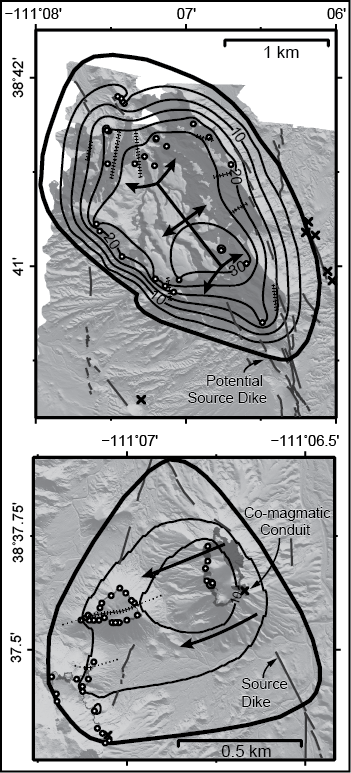
\includegraphics[width=0.4\linewidth]{\FigPath/Fig3-models}
\caption[Sill thickness contour plots of Hebes and Central Cedar sills]{Sill thickness contour plots of Hebes (top) and Central Cedar (bottom) sills. White circles show measurement locations; X symbols are mapped conduits; gray lines are dikes; shaded areas are mapped sills. Thick lines with arrows indicate inferred direction of magma injection; hashed and dotted lines indicate mapped and inferred vertical sill offsets, respectively. Thick contours mark modeled sill boundaries where thickness is modeled to be 0~m.}
\label{fig_twomodels}
\end{figure}

\subsection{Hebes Sill}

The sill at Hebes Mountain (Figure \ref{fig_map}) is primarily preserved as a single 1.9 km$^2$ sill exposed over an area of $\sim$4~km$^2$. This sill generally dips with strata 1$^{\circ}$-8$^{\circ}$ to the northwest, although locally some areas dip 5$^{\circ}$-30$^{\circ}$ toward the center of the sill. Sill thicknesses are measured to a precision of $\pm$75~cm, with virtually all exposures measuring $>$19~m. The sill thins monotonically from the center to the edges of Hebes Mountain, thinning most rapidly to the southwest.

By modeling Hebes sill as a 5.4~km$^2$ area, roughly following the shape of Hebes Mountain, the volume is estimated to be $8.5\times 10^{-2}$ km$^3$. The elongate nature of this sill model (Figure \ref{fig_twomodels}), with increased thickness trending in the northwest dip direction is aligned in the regional dike direction, perhaps indicating a linear source region (dike) feeding the sill.

\subsection{Central Cedar Sill}

\begin{figure}
\centering
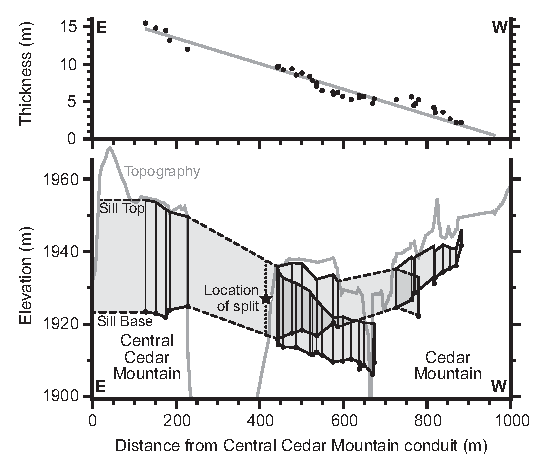
\includegraphics[width=0.5\linewidth]{\FigPath/Fig4-chart}
\caption[Chart of measured thicknesses and elevations of Central Cedar sill]{Top: Measured thicknesses of Central Cedar sill with respect to distance from conduit on Central Cedar Mountain with superimposed linear trend. All vertical errors are within size of plotted points. Bottom: Pseudo–cross section of Central Cedar sill superimposed on current topographic profile. Filled circles represent measured basal elevation (m above sea level) of sill; shaded area represents interpolated sill. Dotted line (star symbol) is inferred location where sill splits into two branches, manifested as step-ups in outcrop.}
\label{fig_chart}
\end{figure}

The Central Cedar sill caps two buttes to the east of Cedar Mountain and is exposed on the east facing cliffs of Cedar Mountain (Figure \ref{fig_panorama}). The outcrops are interpreted to be parts of a single sill, as their basal contacts project across the small valleys between each exposure at the same elevation. Measured thicknesses of the Central Cedar Sill are 2-15 m, with basal contacts that dip with sedimentary host rock, at 2-5$^{\circ}$ WNW to SW. The sill outcrops adjacent to a conduit associated with a $\sim$2~km long dike on Central Cedar Mountain. Basalt between the conduit and sill appears continuous, with no brecciation, suggesting the dike and sill were formed cotemporally, and were thus comagmatic.

The average uncertainty in thickness measurements for Central Cedar Sill is $<$20 cm, due to coverage from both ALSM and TLS data sets. The point cloud also enables the mapping of curvilinear ``step-up'' features, defined by \citet{gartner1986geometry} as vertical offsets between different intrusion pathways, or feathers. Flow direction during intrusion is interpreted to be parallel to step-ups. Step-ups in this sill indicate flow to the W-WNW, away from and/or toward, the conduit. Modeling this sill as a tongue-shaped body intruding to the west from the suspected source dike (Fig S1, top center), Central Cedar Sill has an areal extent of $\sim$0.88~km$^2$, and a total volume of $4.4\times 10^{-3}$~km$^3$ (Table \ref{tab_mappedmodeled}).

A linearly thinning trend away from the conduit is evident in the sill, continuing for 1~km to the observed sill limit (Figure \ref{fig_chart}). Within 100~m of the conduit, sill thickness changes dramatically due to the presence of rotated sandstone blocks with thin basalt lenses injected over the tops of the sandstone blocks, indicating roof collapse into the sill (Figure \ref{fig_panorama}). From these observations we conclude that the Central Cedar Sill was fed from a single dike and was emplaced in a tongue-like fashion to the west in its initial dipping direction. Further, we infer that a conduit-forming volcanic event may have halted further advance of the sill and subsequent flow of magma from the sill into the conduit caused the observed conduit-adjacent roof collapse.

\begin{table}
\centering
\caption{Igneous Material Contributions in the Study Area}
\begin{tabular}{l c c c}
\toprule
 & Area (km$^2$) & Volume  & Vol\% of  \\
 & & (km$^3$) & intrusives \\
\midrule
 Sills & 34.5 & $4.1 \times 10^{-1}$ & 92.9 \\ 
 Dikes & $4.5 \times 10^{-2}$ & $2.2 \times 10^{-2}$ & 5.0 \\
 Conduits & $1.9 \times 10^{-2}$ & $9.5 \times 10^{-3}$ & 2.1 \\
 Total & 34.6 & $4.5 \times 10^{-1}$ & 1.8 \\
 Model Space & 50.0 & 25.0 & --- \\
\bottomrule
\end{tabular}
\label{tab_contribs}
\end{table}

\section{Discussion and Conclusions}

Through lidar mapping of the San Rafael study area, seven sill-forming events in the shallow crust and 12 conduit-forming events have been identified and mapped in detail (Figure \ref{fig_map}). We model the total volume of igneous material stored in sills to be 0.4~km$^3$ within a 25~km$^3$ block. This sill volume represents 93\% of the stored igneous volume in the block, with the remaining 7\% in dikes and conduits. There is no doubt that, volumetrically, sills are a critical component of the magma plumbing system in this distributed volcanic field.

\begin{figure}
\centering
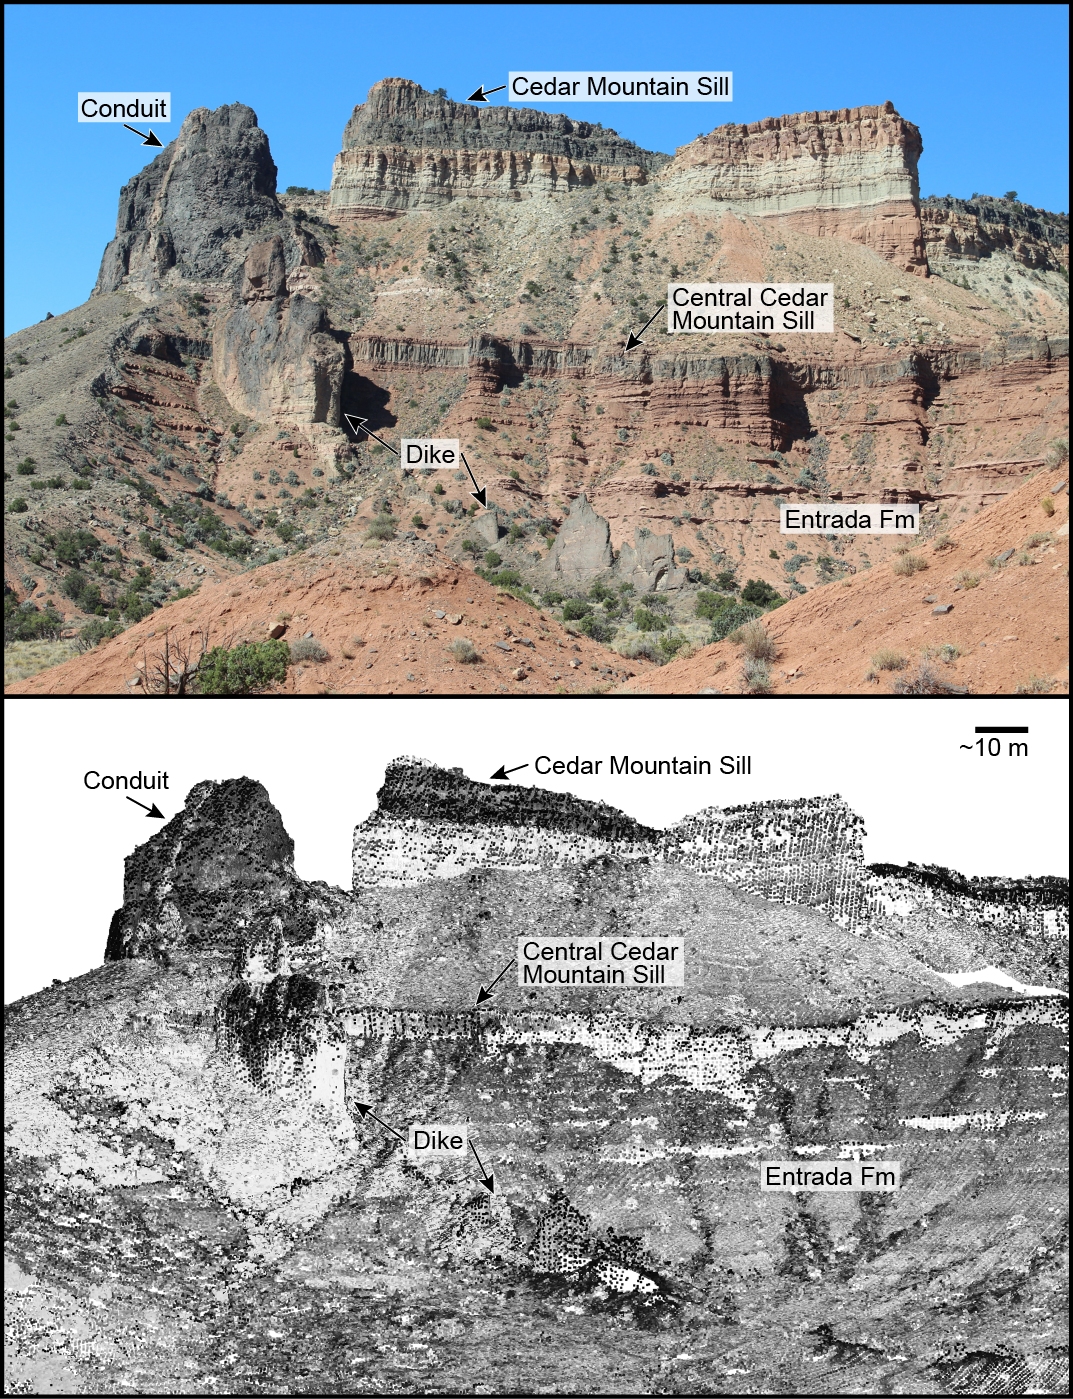
\includegraphics[width=0.7\linewidth]{\FigPath/SFig2-photo_pcloud}
\caption[Photograph and lidar point cloud of the east face of Cedar Mountain]{Top: Photograph of the east face of Cedar Mountain featuring Central Cedar Sill, Cedar Mountain Sill, and a dike which cross-cuts Central Cedar Sill. Sills are separated by dozens of meters by sedimentary rock. Photograph courtesy of J. McIlrath. Bottom: Combined TLS and ALS point cloud of the same view. Near-Infrared intensity differentiates between igneous and sedimentary rocks.}
\label{fig_photo-pcloud}
\end{figure}

It is possible, in fact, that sill volume in the San Rafael Sell volcanic field is comparable to erupted volume. Eruption volumes for the 12 conduits cannot be directly observed, as those lavas are completely eroded away. Eruption volumes for monogenetic volcanoes in similar fields span three orders of magnitude, ranging from 10$^{-3}$ to 10$^{-1}$~km$^3$ \citep[e.g.]{crowe1983aspects, condit1989patterns, kiyosugi2012relationship}. If we assume that average eruption volume is 0.1 km$^3$ for conduits in the San Rafael Swell, $\sim$1.2 km$^3$ of basalt would have been erupted at the surface, four times the estimated sill volume. Again, this comparison suggests that, volumetrically, crustal storage of magma in sills is a major feature of the magmatic system.


\begin{figure}[h!]
\centering
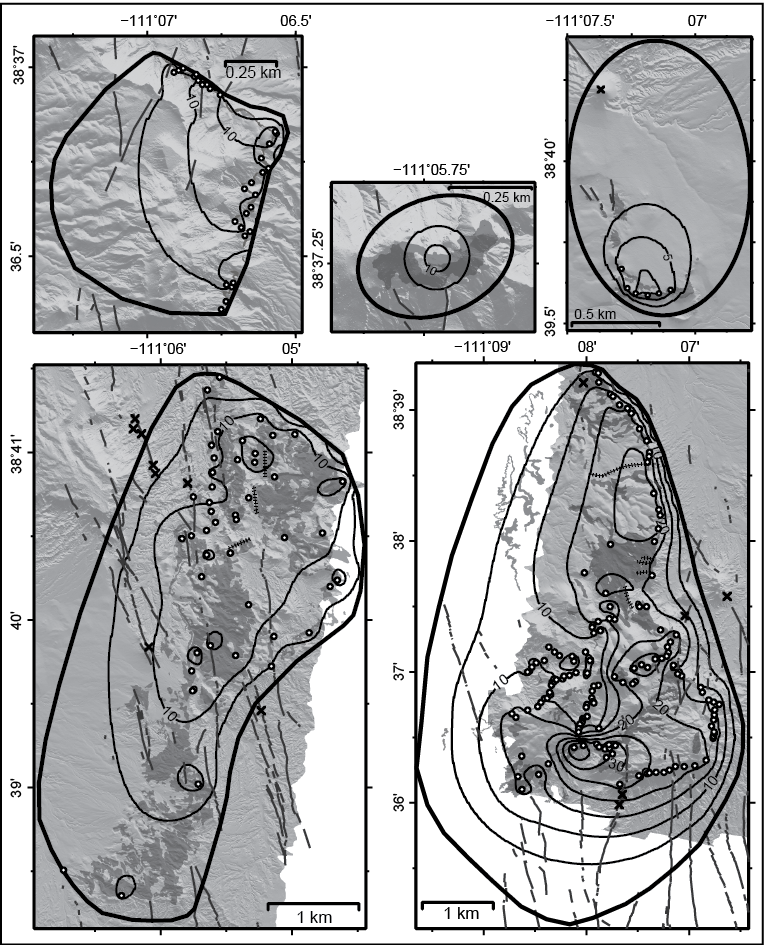
\includegraphics[width=0.7\linewidth]{\FigPath/SFig1-5models}
\caption[Contour plots of thickness models over ALSM hillshade data for additional sills]{Contour plots of thickness models over ALSM hillshade data for additional sills. White circles are measurement locations; Xs are mapped conduits; gray lines are dikes; shaded areas are mapped sills. Thick lines with arrows indicate the inferred direction of magma injection and hashed/dotted lines indicate mapped/inferred vertical sill offsets. Top row, left to right sills are: Lower Cedar, East Cedar Mountain, Razor's; Bottom row, left to right: Bad Luck, Cedar Mountain. Contour intervals are 5~m thickness except Razor’s sill where contours are every 2.5~m. Thick contours mark the modeled sill boundaries where sill thickness is modeled to be 0~m thickness. Note change in map scale. }
\label{fig_fivemodels}
\end{figure}

The general shape of the mapped sills in this field does include a thick center of several to tens of meters in height, tapering edges, and horizontal dimensions of one to several kilometers. While smaller sills exhibit a monotonic decrease in thickness from their interiors (Figure \ref{fig_chart}), the thickness profiles of larger sills are more complex and multiple thickened zones exist (Figure \ref{fig_fivemodels}). The irregular shapes and size range of these sills might suggest that all sills in this area are the product of single injection events and are not polygenetic \citep{gudmundsson2012magma}. Furthermore, the maximum observed thicknesses of each of these sills are not highly correlated to the exposed or modeled areas of each sill. Sills in this area generally ascend stratigraphy only after lifting the roof, enabling exploitation of new bedding planes, suggesting that initial emplacement at this depth was a pressure-driven process, similar to the intrusion of the Trachyte Mesa laccolith (Henry Mountains, Utah, USA) \citep{wetmore2009geometry}. Because horizontal deviatoric stress was low in this area during the Pliocene \citep{delaney1986field}, the minimum compressive stress direction could have significantly migrated from horizontal at 1 km depth, enabling sill formation given local stress conditions influenced by overlying topography \citep{gudmundsson2012magma}.


The development of shallow sills likely affected eruption dynamics. If a comagmatic sill is present during a volcanic eruption, ascending bubbles can become concentrated in the vertical conduit at the conduit-sill junction by disproportional capture of the liquid phase of a two-phase flow in the horizontal branch \citep{conte2000experimental}. This concentration occurs if overall magma flux is sufficiently low. The presence of the sill, therefore, enables modulation of explosive potential, with low magma flow rates resulting in more explosive activity than if a sill was not present. Following the method of \citet{pioli2009controls}, assuming a magma density of 2800~kg/m$^3$, we calculate the transition flux to be $1.8\times 10^5$~kg/s within the Central Cedar Mountain conduit (diameter 25~m), where lower flux would have concentrated bubbles in the conduit system. As average mass eruption rate for strombolian eruptions is commonly observed to be 10$^3$-10$^5$ kg/s \citep{pioli2009controls}, the presence of sills at the level where H$_2$O exolves critically impacts volcanic hazard.

Sills have been identified as a major instigator of unrest in association with stratovolcanoes \citep[e.g.]{biggs2010stratovolcano,tarasewicz2012magma}, volcanic calderas \citep{macedonio2014sill}, and monogenetic volcanic eruptions \citep{erlund2010compositional}. The observation in the San Rafael Swell that the vast majority of igneous rock at ~1 km depth is contained in sills suggests that similar deformation events may be precursory to volcanic eruptions in some active volcanic fields. Monitoring of active volcanic fields may benefit from use of deformation networks to detect sill emplacement in the shallow crust.



\section{Acknowledgments}
This project would not have been possible without the support of David Phillips and UNAVCO for lidar field equipment and data processing assistance. The TLS data acquisition project was funded by a grant from the National Science Foundation (EAR-0910696). ALS data acquisition and processing was completed by the National Center for Airborne Laser Mapping (NCALM) with funding provided by NSF’s Division of Earth Sciences, Instrumentation and Facilities Program (EAR-1043051). M. Oskin and O. Kreylos of UC Davis are thanked for their help regarding LiDAR Viewer. USF students and faculty, Judy McIlrath, Kaz Mannen, Koji Kiyosugi, James Wilson, Samantha Kinman, and Travis Doering are thanked for field assistance. Helpful comments from K. Cashman, A. Gudmundsson, and an anonymous reviewer improved this manuscript.

%%%%%%%%%%%%%%%%%%%%%
%%References Section
%\section{References}
\nobibliography{dissertation_refs}
\bibliographystyle{apalike} 


\begin{table}[h]
\centering
\caption{Lidar Survey Specifications}
\begin{tabular}{l p{2.5cm} c p{3cm} c p{2.3cm}}
\toprule
Survey Date & Instrument & Camera & Instrument  & Points & Data Format \\
&&& Accuracy/Misfit$^*$ & per m$^2$ &\\
\midrule
June 2010	&	Riegl \mbox{LMS-Z620}	&	Nikon D200	&	10 mm/13 cm standard misfit between tiepoints	&	49	&	XYZRGBI ASCII \\
May 2012	&	Riegl VZ-400	&	Nikon D200	&	5 mm/11 cm standard misfit between tiepoints	&	148	&	XYZRGBI ASCII \\
August 2013	&	Optech Gemini ALTM	&	N/A	&	5-35 cm/5cm interswath misfit	&	
6.25	&	LAS \\
\bottomrule
\multicolumn{6}{p{0.95\linewidth}}{$^*$ Misfit in Riegl point clouds are reported after Georeferencing to WGS84 in RiSCAN Pro 1.8.0.}\\
\end{tabular}
\label{tab_specifications}
\end{table}

\newpage
\twocolumn


%\begin{table}[h]
%\centering
\begin{center}
Table 4: Sill Thickness Measurements made in Lidar Viewer\\
\begin{supertabular}{c c c}%\label{tab_measurements}
%\caption{Sill Thickness Measurements made in Lidar Viewer}\\
\toprule
\multicolumn{3}{c}{\textbf{Cedar Mountain Sill}}	\\ 
Easting$^*$	&	Northing$^*$	&	Thickness	\\ 
\midrule
489663 m	 & 	4274770 m	 & 	21.28$\pm$0.10 m\\ 
489243	 & 	4275170	 & 	16.39$\pm$0.74\\ 
489144	 & 	4275170	 & 	14.35$\pm$0.22\\ 
488668	 & 	4275360	 & 	11.95$\pm$0.15\\ 
488367	 & 	4275650	 & 	18.56$\pm$0.17\\ 
488735	 & 	4276050	 & 	19.51$\pm$0.12\\ 
488524	 & 	4278480	 & 	7.38$\pm$0.49\\ 
488565	 & 	4278470	 & 	1.85$\pm$0.28\\ 
488574	 & 	4278340	 & 	9.08$\pm$0.30\\ 
488736	 & 	4278170	 & 	12.58$\pm$0.21\\ 
488774	 & 	4278140	 & 	13.88$\pm$0.26\\ 
488867	 & 	4278020	 & 	13.42$\pm$0.15\\ 
488979	 & 	4277970	 & 	14.78$\pm$0.13\\ 
489031	 & 	4277900	 & 	15.47$\pm$0.20\\ 
489147	 & 	4277680	 & 	18.52$\pm$0.49\\ 
489249	 & 	4277510	 & 	16.47$\pm$0.28\\ 
489288	 & 	4277350	 & 	17.82$\pm$0.20\\ 
489282	 & 	4277290	 & 	18.27$\pm$0.14\\ 
489258	 & 	4277210	 & 	19.37$\pm$0.38\\ 
489348	 & 	4276770	 & 	24.83$\pm$0.42\\ 
489420	 & 	4276540	 & 	21.68$\pm$0.33\\ 
489438	 & 	4276460	 & 	20.01$\pm$0.52\\ 
489412	 & 	4276270	 & 	22.84$\pm$0.29\\ 
489356	 & 	4276090	 & 	18.12$\pm$0.15\\ 
489322	 & 	4275610	 & 	15.10$\pm$0.05\\ 
489442	 & 	4274840	 & 	16.60$\pm$0.15\\ 
489579	 & 	4274670	 & 	22.89$\pm$0.21\\ 
489538	 & 	4274600	 & 	22.18$\pm$0.18\\ 
489551	 & 	4274520	 & 	23.53$\pm$0.14\\ 
489528	 & 	4274470	 & 	23.81$\pm$0.17\\ 
489456	 & 	4274440	 & 	24.55$\pm$0.10\\ 
489363	 & 	4274430	 & 	27.37$\pm$0.15\\ 
489257	 & 	4274310	 & 	27.51$\pm$0.29\\ 
489173	 & 	4274350	 & 	27.05$\pm$0.15\\ 
489067	 & 	4274300	 & 	26.20$\pm$0.29\\ 
489083	 & 	4274110	 & 	22.68$\pm$0.16\\ 
489046	 & 	4274080	 & 	22.26$\pm$0.15\\ 
488908	 & 	4274100	 & 	18.50$\pm$0.32\\ 
488790	 & 	4274180	 & 	23.49$\pm$0.21\\ 
488729	 & 	4275170	 & 	24.68$\pm$0.07\\ 
488717	 & 	4275000	 & 	15.07$\pm$0.21\\ 
488560	 & 	4274960	 & 	15.52$\pm$0.16\\ 
488486	 & 	4274910	 & 	14.51$\pm$0.31\\ 
488475	 & 	4274880	 & 	13.79$\pm$0.33\\ 
488499	 & 	4274800	 & 	11.41$\pm$0.32\\ 
488795	 & 	4274990	 & 	20.09$\pm$0.12\\ 
488590	 & 	4274830	 & 	5.90$\pm$0.17\\ 
488379	 & 	4274530	 & 	5.10$\pm$0.15\\ 
488443	 & 	4274410	 & 	2.68$\pm$0.13\\ 
488537	 & 	4273230	 & 	32.87$\pm$0.15\\ 
488571	 & 	4273190	 & 	28.87$\pm$0.16\\ 
488653	 & 	4273160	 & 	33.31$\pm$0.20\\ 
488716	 & 	4273170	 & 	33.71$\pm$0.29\\ 
488710	 & 	4273220	 & 	33.13$\pm$0.28\\ 
488800	 & 	4273210	 & 	32.62$\pm$0.32\\ 
488759	 & 	4273090	 & 	33.61$\pm$0.34\\ 
488673	 & 	4273040	 & 	29.92$\pm$0.31\\ 
488863	 & 	4272660	 & 	27.55$\pm$0.10\\ 
489132	 & 	4272780	 & 	28.60$\pm$0.34\\ 
489249	 & 	4272810	 & 	22.32$\pm$0.23\\ 
489281	 & 	4272820	 & 	26.53$\pm$0.33\\ 
489375	 & 	4272830	 & 	21.53$\pm$0.46\\ 
489486	 & 	4272830	 & 	25.26$\pm$0.46\\ 
489563	 & 	4272860	 & 	20.21$\pm$0.48\\ 
489647	 & 	4272910	 & 	23.20$\pm$0.21\\ 
489772	 & 	4272910	 & 	20.86$\pm$0.30\\ 
489922	 & 	4272920	 & 	21.32$\pm$0.17\\ 
490081	 & 	4273000	 & 	21.64$\pm$0.10\\ 
490130	 & 	2473110	 & 	18.55$\pm$0.57\\ 
490180	 & 	4273310	 & 	17.58$\pm$0.21\\ 
490186	 & 	4273340	 & 	12.63$\pm$0.11\\ 
490198	 & 	4273380	 & 	23.08$\pm$0.43\\ 
490194	 & 	4273400	 & 	18.06$\pm$0.13\\ 
490158	 & 	4273480	 & 	17.68$\pm$0.28\\ 
490189	 & 	4273570	 & 	18.70$\pm$0.31\\ 
490197	 & 	4273640	 & 	15.89$\pm$0.52\\ 
490206	 & 	4273710	 & 	13.05$\pm$0.35\\ 
490268	 & 	4273790	 & 	13.68$\pm$0.46\\ 
490191	 & 	4273820	 & 	14.27$\pm$0.32\\ 
490121	 & 	4273850	 & 	14.66$\pm$0.10\\ 
490030	 & 	4273960	 & 	13.01$\pm$0.30\\ 
490007	 & 	4274030	 & 	9.51$\pm$0.45\\ 
489738	 & 	4274190	 & 	15.53$\pm$0.12\\ 
489683	 & 	4274220	 & 	17.17$\pm$0.11\\ 
489622	 & 	4274340	 & 	12.12$\pm$0.14\\ 
488560	 & 	4274060	 & 	5.60$\pm$0.24\\ 
488499	 & 	4274050	 & 	6.00$\pm$0.21\\ 
488474	 & 	4273980	 & 	5.63$\pm$0.14\\ 
488468	 & 	4273880	 & 	5.34$\pm$0.11\\ 
488485	 & 	4273830	 & 	4.63$\pm$0.15\\ 
488497	 & 	4273810	 & 	5.91$\pm$0.09\\ 
488399	 & 	4273790	 & 	6.38$\pm$0.26\\ 
488388	 & 	4273750	 & 	6.87$\pm$0.41\\ 
488401	 & 	4273620	 & 	6.85$\pm$0.29\\ 
488340	 & 	4273590	 & 	7.07$\pm$0.21\\ 
488335	 & 	4273560	 & 	8.97$\pm$0.26\\ 
488328	 & 	4273530	 & 	7.77$\pm$0.22\\ 
488297	 & 	4273510	 & 	9.19$\pm$0.18\\ 
488282	 & 	4273450	 & 	8.85$\pm$0.10\\ 
488279	 & 	4273400	 & 	9.19$\pm$0.22\\ 
488567	 & 	4273450	 & 	9.62$\pm$0.37\\ 
488218	 & 	4273180	 & 	40.57$\pm$0.15\\ 
488347	 & 	4273210	 & 	40.70$\pm$0.21\\ 
487479	 & 	4272590	 & 	16.55$\pm$0.26\\ 
487422	 & 	4272770	 & 	15.22$\pm$0.05\\ 
487851	 & 	4272950	 & 	17.97$\pm$0.24\\ 
487715	 & 	4272800	 & 	12.68$\pm$0.14\\ 
487476	 & 	4273060	 & 	17.94$\pm$0.28\\ 
487395	 & 	4273610	 & 	19.54$\pm$0.19\\ 
487339	 & 	4273660	 & 	15.05$\pm$0.52\\ 
487561	 & 	4273710	 & 	13.93$\pm$0.61\\ 
487705	 & 	4273760	 & 	12.85$\pm$0.67\\ 
487749	 & 	4273820	 & 	12.20$\pm$0.36\\ 
487796	 & 	4273870	 & 	12.40$\pm$0.36\\ 
487838	 & 	4273880	 & 	8.61$\pm$0.23\\ 
487885	 & 	4273930	 & 	9.51$\pm$0.46\\ 
487872	 & 	4273960	 & 	9.87$\pm$0.44\\ 
487897	 & 	4274060	 & 	10.22$\pm$0.49\\ 
487936	 & 	4274110	 & 	8.76$\pm$0.17\\ 
487933	 & 	4274150	 & 	10.36$\pm$0.41\\ 
487967	 & 	4274140	 & 	8.97$\pm$0.32\\ 
488056	 & 	4274150	 & 	7.81$\pm$0.57\\ 
488074	 & 	4274190	 & 	6.97$\pm$0.34\\ 
488153	 & 	4274200	 & 	6.45$\pm$0.33\\ 
488244	 & 	4274240	 & 	7.56$\pm$0.23\\ 
488405	 & 	4274230	 & 	4.15$\pm$0.35\\ 
488216	 & 	4274400	 & 	17.30$\pm$0.15\\ 
488190	 & 	4274470	 & 	9.90$\pm$0.44\\ 
488011	 & 	4274480	 & 	6.16$\pm$0.28\\ 
487943	 & 	4274530	 & 	6.22$\pm$0.27\\ 
487863	 & 	4274600	 & 	5.83$\pm$0.11\\ 
487798	 & 	4274410	 & 	8.82$\pm$0.22\\ 
487683	 & 	4274380	 & 	10.90$\pm$0.36\\ 
487624	 & 	4274320	 & 	10.12$\pm$0.44\\ 
487562	 & 	4274250	 & 	8.39$\pm$0.22\\ 
\\
\toprule
\multicolumn{3}{c}{\textbf{Central Cedar Mountain Sill}}	\\ 
Easting	&	Northing	&	Thickness	\\ 
\midrule
489772 m	 & 	4274800 m	 & 	3.54$\pm$0.03 m\\ 
489756	 & 	4274790	 & 	3.61$\pm$0.04\\ 
489745	 & 	4274830	 & 	4.26$\pm$0.04\\ 
489724	 & 	4274850	 & 	4.10$\pm$0.16\\ 
489887	 & 	4275310	 & 	9.61$\pm$0.11\\ 
489875	 & 	4275360	 & 	9.77$\pm$0.30\\ 
489863	 & 	4275370	 & 	9.25$\pm$0.22\\ 
489840	 & 	4275400	 & 	9.38$\pm$0.25\\ 
489816	 & 	4275420	 & 	8.84$\pm$0.02\\ 
489781	 & 	4275390	 & 	7.52$\pm$0.42\\ 
490174	 & 	4275590	 & 	12.02$\pm$0.08\\ 
490174	 & 	4275530	 & 	13.22$\pm$0.10\\ 
490193	 & 	4275440	 & 	15.53$\pm$0.12\\ 
489688	 & 	4275050	 & 	5.27$\pm$0.13\\ 
489664	 & 	4275000	 & 	4.73$\pm$0.16\\ 
489710	 & 	4275120	 & 	5.37$\pm$0.21\\ 
489640	 & 	4275050	 & 	4.47$\pm$0.29\\ 
489538	 & 	4275060	 & 	2.71$\pm$0.33\\ 
489557	 & 	4274990	 & 	2.20$\pm$0.14\\ 
489560	 & 	4274960	 & 	2.23$\pm$0.38\\ 
489808	 & 	4275280	 & 	7.85$\pm$0.20\\ 
489784	 & 	4275280	 & 	6.49$\pm$0.16\\ 
489753	 & 	4275300	 & 	6.32$\pm$0.13\\ 
489731	 & 	4275290	 & 	5.75$\pm$0.09\\ 
489710	 & 	4275290	 & 	5.28$\pm$0.26\\ 
489691	 & 	4275290	 & 	5.52$\pm$0.22\\ 
489678	 & 	4275300	 & 	5.72$\pm$0.15\\ 
489658	 & 	4275290	 & 	4.78$\pm$0.23\\ 
489743	 & 	4275360	 & 	5.98$\pm$0.43\\ 
489735	 & 	4275340	 & 	6.21$\pm$0.17\\ 
489687	 & 	4275310	 & 	5.82$\pm$0.66\\ 
489845	 & 	4275290	 & 	8.57$\pm$0.20\\ 
489814	 & 	4275280	 & 	8.38$\pm$0.14\\ 
489798	 & 	4275280	 & 	7.08$\pm$0.17\\ 
489712	 & 	4274920	 & 	5.26$\pm$0.18\\ 
489663	 & 	4275020	 & 	5.62$\pm$0.17\\ 
490165	 & 	4275500	 & 	14.55$\pm$0.31\\ 
490170	 & 	4275450	 & 	14.87$\pm$0.10\\ 
\\
\toprule
\multicolumn{3}{c}{\textbf{Razor's Sill}}	\\ 
Easting	&	Northing	&	Thickness	\\ 
\midrule
489464 m	 & 	4279070 m	 & 	5.7$\pm$0.11 m\\ 
489511	 & 	4279040	 & 	7.78$\pm$0.18\\ 
489580	 & 	4279030	 & 	7.25$\pm$0.08\\ 
489644	 & 	4279040	 & 	7.78$\pm$0.10\\ 
489710	 & 	4279060	 & 	5.81$\pm$0.11\\ 
489431	 & 	4279180	 & 	6.33$\pm$0.15 \\
\\ 
\toprule
\multicolumn{3}{c}{\textbf{Hebes Sill}}	\\ 
Easting	&	Northing	&	Thickness	\\ 
\midrule
490593 m	 & 	4281090 m	 & 	22.58$\pm$0.16 m\\ 
490439	 & 	4281670	 & 	33.34$\pm$0.42\\ 
490194	 & 	4281800	 & 	36.08$\pm$0.10\\ 
490290	 & 	4282640	 & 	22.49$\pm$0.15\\ 
489926	 & 	4283040	 & 	24.07$\pm$0.32\\ 
490078	 & 	4282910	 & 	23.27$\pm$0.36\\ 
489565	 & 	4282890	 & 	26.61$\pm$0.18\\ 
489110	 & 	4282970	 & 	19.77$\pm$0.21\\ 
489020	 & 	4281990	 & 	20.72$\pm$0.20\\ 
489234	 & 	4281740	 & 	20.80$\pm$0.23\\ 
489558	 & 	4281520	 & 	27.48$\pm$0.34\\ 
489651	 & 	4281450	 & 	27.57$\pm$0.31\\ 
489786	 & 	4281510	 & 	30.38$\pm$0.30\\ 
489736	 & 	4281390	 & 	22.64$\pm$0.34\\ 
488987	 & 	4282060	 & 	27.73$\pm$0.14\\ 
489096	 & 	4282650	 & 	21.33$\pm$0.29\\ 
489359	 & 	4282650	 & 	28.24$\pm$0.29\\ 
489453	 & 	4282720	 & 	25.33$\pm$0.14\\ 
489550	 & 	4282630	 & 	27.77$\pm$0.23\\ 
489668	 & 	4282820	 & 	27.80$\pm$0.41\\ 
489568	 & 	4282900	 & 	27.01$\pm$0.35\\ 
489258	 & 	4283240	 & 	4.51$\pm$0.30\\ 
489242	 & 	4283260	 & 	3.50$\pm$0.35\\ 
489228	 & 	4283290	 & 	7.30$\pm$0.29\\ 
489196	 & 	4283310	 & 	7.55$\pm$0.64\\ 
489089	 & 	4282980	 & 	21.65$\pm$0.47\\ 
\\ 
\toprule
\multicolumn{3}{c}{\textbf{Bad Luck Sill}}	\\ 
Easting	&	Northing	&	Thickness	\\ 
\midrule
492071 m	 & 	4280530 m	 & 	14.37$\pm$0.17 m\\ 
492785	 & 	4281840	 & 	15.32$\pm$0.12\\ 
491954	 & 	4282470	 & 	5.64$\pm$0.43\\ 
491820	 & 	4282330	 & 	4.81$\pm$0.20\\ 
491866	 & 	4281720	 & 	9.18$\pm$0.21\\ 
491892	 & 	4281580	 & 	7.93$\pm$0.25\\ 
492152	 & 	4281560	 & 	14.03$\pm$0.39\\ 
492342	 & 	4281530	 & 	16.49$\pm$0.38\\ 
492560	 & 	4281370	 & 	13.22$\pm$0.26\\ 
492275	 & 	4281140	 & 	12.17$\pm$0.29\\ 
493087	 & 	4280750	 & 	13.74$\pm$0.26\\ 
492940	 & 	4279650	 & 	8.36$\pm$0.32\\ 
492126	 & 	4280950	 & 	9.93$\pm$0.33\\ 
492137	 & 	4280900	 & 	11.57$\pm$0.36\\ 
491933	 & 	4281870	 & 	8.93$\pm$0.34\\ 
491641	 & 	4280720	 & 	11.42$\pm$0.27\\ 
491537	 & 	4280690	 & 	15.79$\pm$0.14\\ 
491753	 & 	4280270	 & 	13.25$\pm$0.30\\ 
492071	 & 	4280530	 & 	14.92$\pm$0.21\\ 
491643	 & 	4279230	 & 	13.02$\pm$0.14\\ 
491651	 & 	4279010	 & 	15.66$\pm$0.18\\ 
491713	 & 	4277980	 & 	12.82$\pm$0.17\\ 
490865	 & 	4276750	 & 	6.83$\pm$0.15\\ 
490225	 & 	4277030	 & 	4.03$\pm$0.05\\ 
493252	 & 	4280230	 & 	13.43$\pm$0.34\\ 
493172	 & 	4280160	 & 	7.45$\pm$0.21\\ 
492669	 & 	4280700	 & 	12.08$\pm$0.08\\ 
492551	 & 	4279610	 & 	6.69$\pm$0.14\\ 
492524	 & 	4279280	 & 	5.21$\pm$0.29\\ 
492128	 & 	4279400	 & 	15.28$\pm$0.07\\ 
491851	 & 	4279510	 & 	7.65$\pm$0.21\\ 
491703	 & 	4279430	 & 	17.32$\pm$0.07\\ 
493311	 & 	4281320	 & 	18.52$\pm$0.36\\ 
492541	 & 	4281830	 & 	12.38$\pm$0.11\\ 
492404	 & 	4282010	 & 	12.20$\pm$0.24\\ 
492346	 & 	4281630	 & 	18.96$\pm$0.17\\ 
492205	 & 	4281770	 & 	15.35$\pm$0.14\\ 
491840	 & 	4281090	 & 	9.69$\pm$0.16\\ 
491876	 & 	4281420	 & 	11.09$\pm$0.17\\ 
491871	 & 	4281260	 & 	8.46$\pm$0.28\\ 
491663	 & 	4281150	 & 	9.22$\pm$0.20\\ 
491860	 & 	4280990	 & 	11.12$\pm$0.27\\ 
491907	 & 	4280870	 & 	11.53$\pm$0.19\\ 
491808	 & 	4280780	 & 	12.79$\pm$0.28\\ 
491811	 & 	4280510	 & 	15.74$\pm$0.20\\ 
492272	 & 	4279960	 & 	13.22$\pm$0.12\\ 
\\ 
\toprule
\multicolumn{3}{c}{\textbf{Lower Cedar Mountain Sill}}	\\ 
Easting	&	Northing	&	Thickness	\\ 
\midrule
490227 m	 & 	4273100 m	 & 	1.26$\pm$0.13 m\\ 
490230	 & 	4273180	 & 	6.82$\pm$0.19\\ 
490256	 & 	4273170	 & 	2.26$\pm$0.23\\ 
490263	 & 	4273190	 & 	0.76$\pm$0.08\\ 
490320	 & 	4273420	 & 	9.44$\pm$0.26\\ 
490345	 & 	4273440	 & 	9.19$\pm$0.22\\ 
490302	 & 	4273460	 & 	10.71$\pm$0.35\\ 
490272	 & 	4273490	 & 	12.09$\pm$0.41\\ 
490327	 & 	4273530	 & 	8.57$\pm$0.20\\ 
490350	 & 	4273560	 & 	6.32$\pm$0.43\\ 
490372	 & 	4273620	 & 	10.26$\pm$0.16\\ 
490319	 & 	4273650	 & 	12.62$\pm$0.14\\ 
490353	 & 	4273680	 & 	12.53$\pm$0.44\\ 
490408	 & 	4273730	 & 	10.52$\pm$0.13\\ 
490436	 & 	4273750	 & 	9.95$\pm$0.35\\ 
490401	 & 	4273800	 & 	8.95$\pm$0.23\\ 
490441	 & 	4273870	 & 	12.06$\pm$0.20\\ 
490475	 & 	4273920	 & 	11.19$\pm$0.20\\ 
490469	 & 	4273930	 & 	13.32$\pm$0.18\\ 
490200	 & 	4274110	 & 	12.37$\pm$0.45\\ 
490151	 & 	4274140	 & 	13.21$\pm$0.16\\ 
490136	 & 	4274160	 & 	7.59$\pm$0.25\\ 
490113	 & 	4274160	 & 	14.43$\pm$0.45\\ 
490093	 & 	4274180	 & 	10.50$\pm$0.45\\ 
490073	 & 	4274200	 & 	5.39$\pm$0.19\\ 
490083	 & 	4274210	 & 	3.20$\pm$0.15\\ 
489974	 & 	4274220	 & 	10.40$\pm$0.36\\ 
489997	 & 	4274230	 & 	4.38$\pm$0.26\\ 
490019	 & 	4274240	 & 	2.85$\pm$0.16\\ 
490204	 & 	4273060	 & 	1.88$\pm$0.24\\ 
\bottomrule
\multicolumn{3}{p{0.8\linewidth}}{$^*$ Eastings and northings reported in UTM Zone 12 coordinates.}\\
%\end{tabular}
\end{supertabular}
\end{center}

\onecolumn
